%%%%%%%%%%%%%%%%%%%%%%%%%%%%%%%%%%%%%%%%%
% Simple Sectioned Essay Template
% LaTeX Template
%
% This template has been downloaded from:
% http://www.latextemplates.com
%
% Note:
% The \lipsum[#] commands throughout this template generate dummy text
% to fill the template out. These commands should all be removed when 
% writing essay content.
%
%%%%%%%%%%%%%%%%%%%%%%%%%%%%%%%%%%%%%%%%%

%----------------------------------------------------------------------------------------
%	PACKAGES AND OTHER DOCUMENT CONFIGURATIONS
%----------------------------------------------------------------------------------------

\documentclass[12pt]{article} % Default font size is 12pt, it can be changed here

\usepackage{geometry} % Required to change the page size to A4
\geometry{a4paper} % Set the page size to be A4 as opposed to the default US Letter

\usepackage{graphicx} % Required for including pictures

\usepackage{float} % Allows putting an [H] in \begin{figure} to specify the exact location of the figure
\usepackage{wrapfig} % Allows in-line images such as the example fish picture

\usepackage{lipsum} % Used for inserting dummy 'Lorem ipsum' text into the template

\linespread{1.2} % Line spacing

%\setlength\parindent{0pt} % Uncomment to remove all indentation from paragraphs

\graphicspath{{Pictures/}} % Specifies the directory where pictures are stored

\begin{document}
	
	%----------------------------------------------------------------------------------------
	%	TITLE PAGE
	%----------------------------------------------------------------------------------------
	
	\begin{titlepage}
		
		\newcommand{\HRule}{\rule{\linewidth}{0.5mm}} % Defines a new command for the horizontal lines, change thickness here
		
		\center % Center everything on the page
		
		\textsc{\LARGE Wits University}\\[1.5cm] % Name of your university/college
		\textsc{\Large School of Electrical and Information Engineering}\\[0.5cm] % Major heading such as course name
		\textsc{\large ELEN7046 - Software Technologies and Techniques}\\[0.5cm] % Minor heading such as course title
		
		\HRule \\[0.4cm]
		{ \huge \bfseries Big Data Visualization using Commodity Hardware and Open Source Software}\\[0.4cm] % Title of your document
		
		\HRule \\[0.6cm]
		
		\begin{minipage}
			{0.4
				\textwidth} 
			\begin{flushleft}
				\large \emph{Authors:}\\
				Gareth \textsc{Stephenson} \\
				Matsobane \textsc{Khwinana} \\
				Sidwell \textsc{Mokhemisa} \\
				Dave \textsc{Cloete}\\
				Kyle \textsc{Trehaeven}
			\end{flushleft}
		\end{minipage}
		~ 
		\begin{minipage}
			{0.4
				\textwidth} 
			\begin{flushright}
				\large \emph{Student Number:} \\
				778919 \\
				779053  \\
				1229756 \\
				1573016 \\
				0602877N
				% Supervisor's Name
			\end{flushright}
		\end{minipage}
		\\[1cm]
		
		% Abstract
		\begin{flushleft}\large
			\textsc{Abstract}\\
			The project aims to provide a low cost solution to big data processing problems, enabling a commercially viable option to individuals, small businesses and academia using commodity hardware. This report explores the use of  Open Source technologies Apache Spark and Scala as well as the low cost and scalable Raspberry Pi's. After building a prototype system to source, process and visualize data from twitter, it was concluded that  commodity hardware is a viable small-scale solution to working with Big Data.
			
		\end{flushleft}
		{\large \today}\\[3cm] % Date, change the \today to a set date if you want to be precise
		
		%\includegraphics{Logo}\\[1cm] % Include a department/university logo - this will require the graphicx package
		
		\vfill % Fill the rest of the page with whitespace
		
	\end{titlepage}
	
		% Abstract
		\begin{flushleft}\large
			\textsc{Declaration of Originality}\\
			
			
		\end{flushleft}
	
	%----------------------------------------------------------------------------------------
	%	TABLE OF CONTENTS
	%----------------------------------------------------------------------------------------
	
	\tableofcontents % Include a table of contents
	
	\newpage % Begins the essay on a new page instead of on the same page as the table of contents 
	
	%----------------------------------------------------------------------------------------
	%	INTRODUCTION
	%----------------------------------------------------------------------------------------
	
	\section{Introduction} % Major section
	
This report presents the work done by Group 2 in response to the project brief for ELEN7046: Software Technologies and Techniques.\\

The report will broadly focus on the following topics:

\begin{itemize}
	\item The Methodology followed to execute the project;
	\item The Architecture of the solution developed for the project; and
	\item The different technologies used to deliver the solution.
\end{itemize}

\subsection{Problem Statement}

There is an abundance of big data available to individuals and companies with very limited capacity to refine this data into meaningful information, particularly for small scale endeavours. Big Data processing is often locked behind high cost barriers to entry, and individuals, start ups and academics may find it difficult to be involved in Big Data processing.

\subsection{Solution Summary}

Commodity hardware is available to provide a means by which the barrier to entry for Big Data projects can be overcome. Simple, low cost components can be leveraged to address each of the parts of a big data processing solution, whether it be data sourcing, transormation, or visualization; and can be scaled according to needs or as required.

\subsection{Approach}

%\subsubsection{Methodology}
	
		%\subsection{Executive Summary} % --optional
		
		%------------------------------------------------
		
	\section{Literature Review}
	
	\subsection {Data Sourcing}
	
	This project was intended to deliver a system or solution for the visualization of Big Data. For this reason it is important that we start by defining what Big Data is.
	\\
	According to Maden[1], Big Data can be defined as "data that is too big, too fast, or too hard for existing tools to process."
	\\
	The above definition further supports our group's decision to focus on Twitter as the source of data for the project. Statistics have shown the following average figures with regards to the amount of data that one can get from Twitter[2]:
	\\
	
		\begin{itemize}
			\item 6000 per second; 
			\item 350 000 per minute;
			\item 500 million per day; and
			\item 200 billion in a year.
		\end{itemize}
	
	\subsection {Big Data Processing Algorithm}
	
	The team sought to have all the processing of the Big Data received from Twitter done on multiple nodes following the principles of MapReduce.
	\\
	\\
	Apache Spark was used for this project together with MapReduce which in the main delivers the MapReduce functionality based on the algorithm that is broken down into the Mapper class and the Reducer class[3].

		%--Where they come from
		%--What they currently do
		%--General experience
	
	%Example citation \cite{Figueredo:2009dg}.
	
	%------------------------------------------------
	
	%\subsection{Description of Acronyms} % Sub-section
	
	%IS - Information Systems \\
	
	%------------------------------------------------
	%Sample image for future reference (image to be taken out)
	%\begin{figure}[H] % Example image
	%\center{
\includegraphics[width=0.5\linewidth]{placeholder}}
	%\caption{Example image.}
	%\label{fig:speciation}
	%\end{figure}
	
	%------------------------------------------------
	%-------------
	%	MAJOR SECTION 1
	%----------------------------------------------------------------------------------------
	
	%\section{Problem Statement}
	
	
	
	%\subsection{Executive Summary} % --optional
	
	%------------------------------------------------
	
%	\subsection{Data Collection}
	%--Where they come from
	%--What they currently do
	%--General experience
	
	
	
	%------------------------------------------------
	
%	\subsection{Data Processing}
	


	%--Risk categories SP03
	
%	\subsubsection{Cost and Schedule}
	
	
	
	%--Earn Value Management SP01
	
	
	%--Earn Value Management SP01
	
%	\subsection{Data Visualization}
	

	%--Summary of the above
	%--Kill project/replace project manager/continue project???
	
	%------------------------------------------------
	
	\section{Lifecycle Methodology}
	
	%\subsection{Explanation Summary} %--optional
	
	%------------------------------------------------
	In order for the team to successfully deliver this project, a development methodology based on IBM Rational Unified Process (RUP) was followed albeit tailored to cater for the specific needs of this project.\\
	\\
	The diagram below depicts the IBM RUP model:
	
		\begin{figure}[H] % Example image
			\center{\includegraphics[width=1.15\linewidth]{ibm1}}
			\caption{IBM Rational Unified Process (Source: RUP, Best Practices for Software Development Teams)}
			\label{fig:speciation}
		\end{figure}
		
		
	
%	\subsection{info}
	
	
	%------------------------------------------------
	
%	\subsection{Observation} % Sub-section
	
	
%	\subsubsection{Value}
	
	
	%\\subsubsection{Risk}
	%--Risk categories SP03

%	\subsubsection{Cost \& Schedule}
	

	
	%\subsection{xxx}
	\section{Assumptions and Constraints}
	
	Early ideas in the project were based on the Twitter location data; for example, in the inception one of the project the first idea was to visualise the world's reaction to Oscar Pistorious' murder accussation over the world map. Given this idea, the location at which each Twitter postings (tweets) were made was paramount to the success of that idea. Unfortunately due the amount of Twitter data found on this subject, the team decided it was not big enough to qualify as Big Data. The project then decided to rather visualise the currently most topical of subjects, the upcoming United States general elections and also the upcoming South African municipal elections. The idea of using locations where tweets were posted stuck with the project. 
	\\
	\\
	However, during the data collection exercise it was discovered that most of the Twitter posts (tweets) had no location data attached to them. It turns out most Twitter users disable their GPS sensor for the Twitter application, presumably for security and privacy reasons. This meant the project would collect data that did not have locations and that would sabotage ideas of visualising data based on locations. After a further analysis on the Twitter data that can be collected, the team came to a realisation that Twitter users have profile location data specified as a free text. As a workaround the user profile location was collected alongside the tweets. Therefore each tweet that did not have a location, the user profile location data was associated with that tweeet.The assumption being made by the project was that location of each tweet is the same as that of the user's profile. The project acknowledges that if the user's GPS sensor is turned on, profile location may not necessarily be the same as the location at which the tweet would be posted.
	\\
	\\
	Both Twitter and Google API have usage limits which presented a constraint to the project. Twitter search API allows returns 100 tweets per request and allows only 450 requests per 15 minute window [1]. Only 2500 requests per day are allowed by the standard Google Maps Geocoding API [2].\\
	\\
	%Assumptions - Kyle
		We assume a rudimentary algorithm for sentiment assessment is "Good Enough", forgoing complex natural language inference.\\
		We assume that any incidental tweets sourced (such as EFF = Electronic Freedom Foundation) are minimal and acceptable.\\
		We assume that Twitter is providing us with either the full extent of our search criteria, or if this is not the case, then the sample we receive is a representational slice.\\
		We assume information that users provide on twitter (name of their location in particular) is correct and relevant, and that those who do not are in the minority.\\
		Failing the above, we assume that of those who do provide location based information, their distribution is representative of the norm.\\
		We acknowledge that our demographics are skewed (younger people more likely to use twitter, poorer South Africans less likely to use twitter).\\
		We acknowledge that application software is not flawlessly optimised.
		
	
		%\subsection{Tweet Locations}
	%	The group encountered tweet location issues. \\
		\subsection{Pros and Cons determinations}
		Rudimentary algorithm for determining Twitter statements (tweets) that are against or for a particular candidate was adopted... 
	%------------------------------------------------
	\section {Design Decisions}
	
	The table below details all the key design decisions made in the delivery of the solution:
	
\begin{itemize} 
	\item \textbf{History Data:} History data/ batch interface to Twitter was designed to provide past data subscribed to based on date range.
	
	\item \textbf{Streaming Data:} 
	This interface provides for all subscribed data in real-time starting from now and going into the future.
	
	\item \textbf{GoogleMaps:} 
	Tweet location was derived from the co-ordinates found in a tweet where the person tweeting enabled location services on their device to provide current location information. Where privacy settings were not enabled for current location, an interface to GoogleMaps was developed to read the location information of the person tweeting from their Twitter profile and resolve this to actual co-ordinates.
	
	\item \textbf{Security Directive(s):} 
	It was decided that where security is concerned, only the Twitter and GoogleMaps security requirements be adhered to where integration is concerned. All data acquired from Twitter is data that is already in the public domain, therefore no effort was required to secure the data while in transit, hence the use of only FTP instead of a lot more secure transport mechanism.
\end{itemize}
	
	
	
	%\subsection{Explanation Summary} %--optional

	%------------------------------------------------
	
	%--Earn Value Management 
	
	
	%--Summary of the above
	%--Kill project/replace project manager/continue project???

	
	
	%-----------------------------------------------
	
	\section{Success Criteria} % Major section
	
	\begin{itemize}
		\item Build a system that uses commodity hardware to solve for big data problems;
		\item Provide a solution that covers the data sourcing, transformation and presentation of social media data from Twitter relating to the United States and South African elections. The end result must be visualization that provides insight to the sentiment of election candidates on Twitter.
	\end{itemize}
	
	
	
	\section{Solution Design}
		
	\subsection{High Level Design: Component Architecture}
	The high level component model below depicts the key features of the solution delivered for the project.
	\\
	\\
	This design can be categorised into the following three features from a functionality point of view:
	
		\begin{itemize}
			\item Acquiring data from Twitter based on topics subscription - Political Party sentiment in USA and RSA for 2016. This was achieved by using JEE for history and C\# for online data acquisition while persisting all data in MongoDB.
			\item Data processing was achieved using Apache Spark with MapReduce algorithms developed in Scala. Data in MongoDB was extracted and FTP'd to our clustered infrastructure where all the necessary transformation happened.
			\item Extracts from the transformation process were sent to the presentation tier application in JSON format where node.js was used in conjunction with D3 chartz to render the visualized big data content on a web browser.
		\end{itemize}
	
	
		\begin{figure}[H] % Example image
			\center{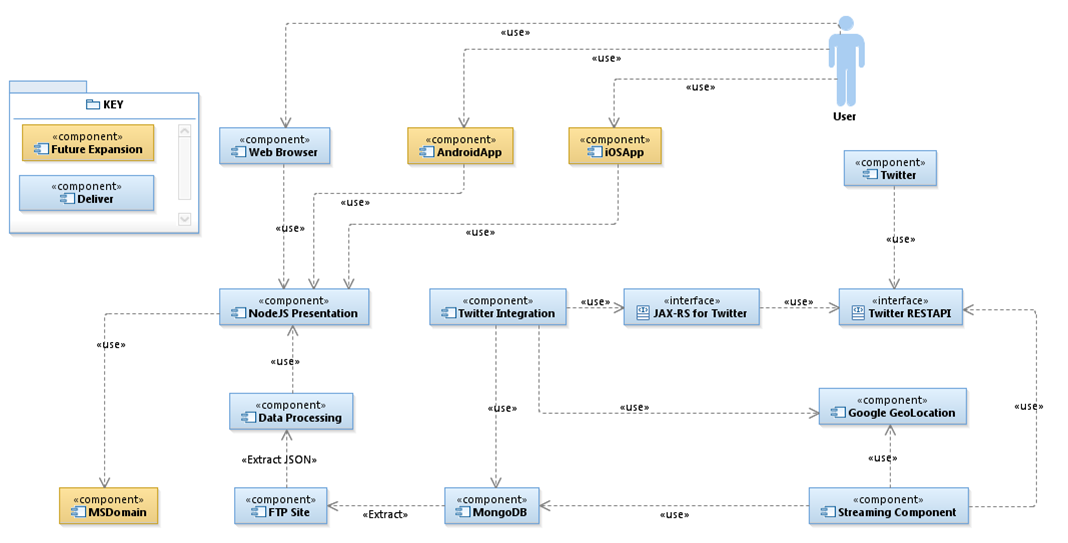
\includegraphics[width=1.15\linewidth]{HLD1}}
			\caption{High Level Component Model.}
			\label{fig:speciation}
		\end{figure}
	
	\subsection{Detailed Designs}
	
	\subsubsection{Data Acquisition (Batch)}
	
		\begin{figure}[H] % Example image
			\center{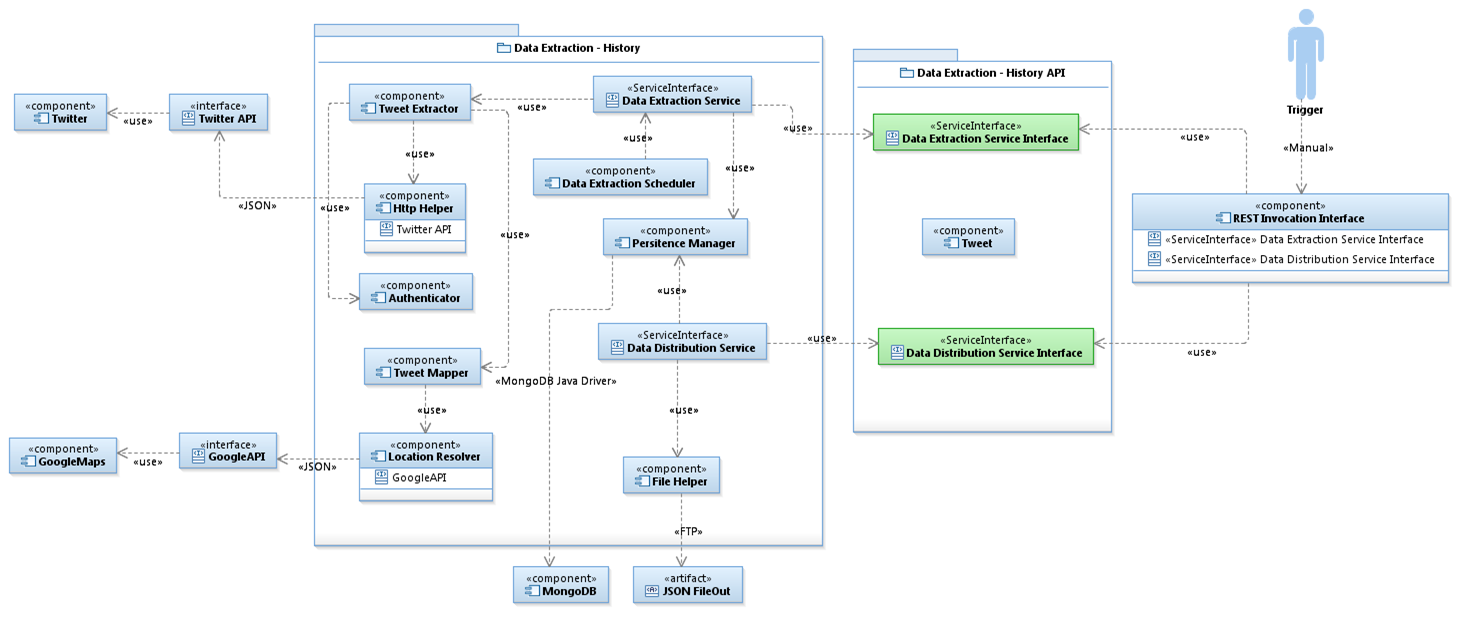
\includegraphics[width=1.15\linewidth]{Batch}}
			\caption{Component Model: Streaming Module}
			\label{fig:speciation}
		\end{figure}
	
	\subsubsection{Data Acquisition (Streaming)}
	
		\begin{figure}[H] % Example image
			\center{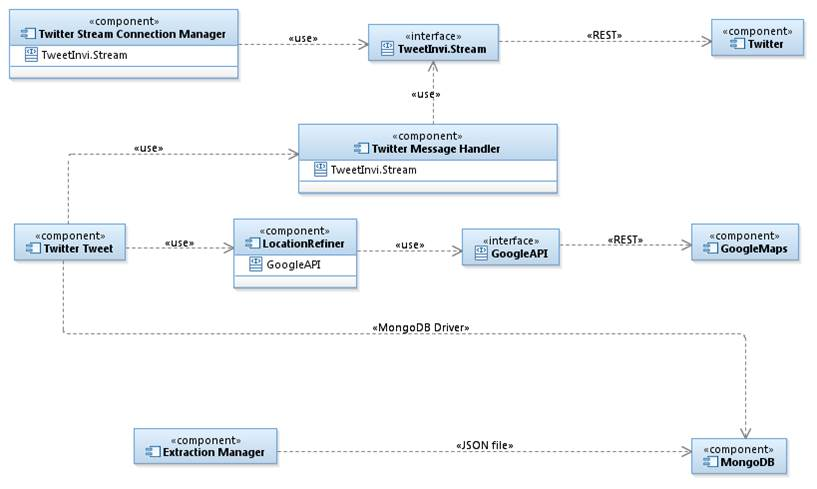
\includegraphics[width=1.15\linewidth]{Streaming}}
			\caption{Component Model: Streaming Module}
			\label{fig:speciation}
		\end{figure}
	
	\subsubsection{Data Processing}
	
	\begin{figure}[H] % Example image
		\center{\includegraphics[width=1.15\linewidth]{MapReduce}}
		\caption{Context Diagram: Data Processing}
		\label{fig:speciation}
	\end{figure}
	
	\subsubsection{Data Visualization}
	
	The Visual component implements the MVC pattern to separate the View and controlling logic from the Data. This allows for the data components to be develop separately from the Views. Between the Views and Data Models where Controllers responsible to load the views based on the set configuration and provide the views with the required data model.\\
	\\
	The Data Visualisation component was designed to be agnostic of the content and allows for comparison of categories in a topic agnostic of the topic or categories.
	All charts were design to be scalable. All graphs will render as the view point change allowing for a pleasant user experience.
	
	
		\begin{figure}[H] % Example image
			\center{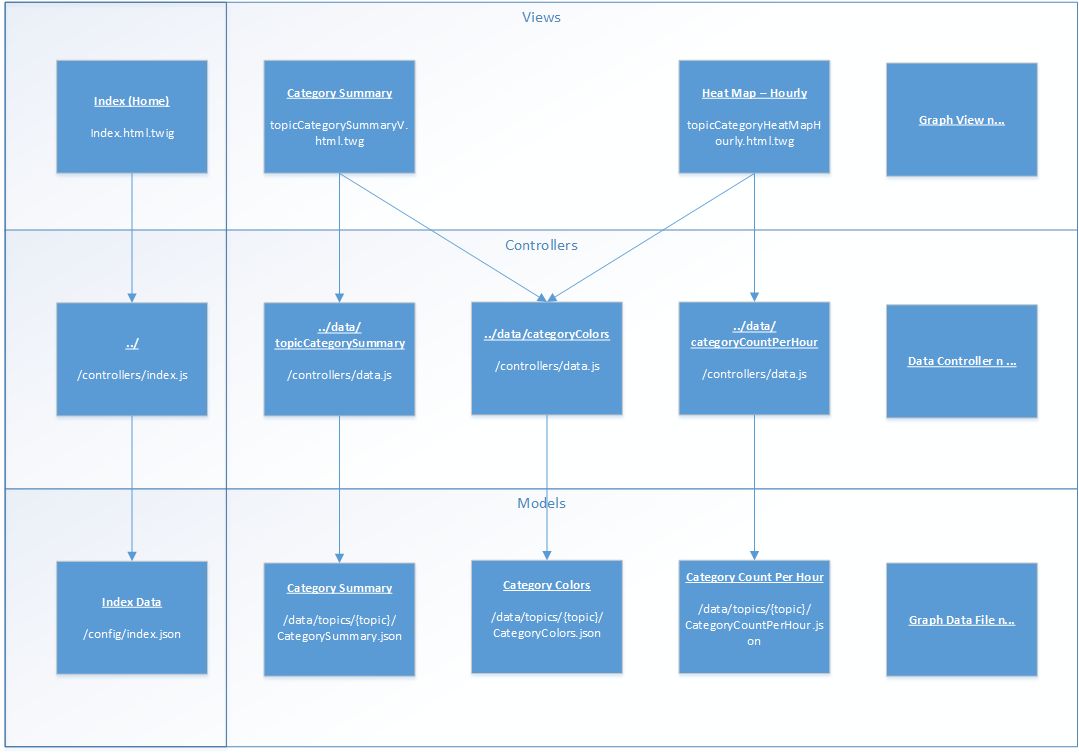
\includegraphics[width=1.15\linewidth]{Visual}}
			\caption{Visualization: MVC Framework}
			\label{fig:speciation}
		\end{figure}
	
	\subsection{Operational Model: Infrastructure Design}
	
	The Raspberry Pi environment is limited in system resources, specifically RAM. It only has 1GB of RAM which is partitioned for use between the system (accessible by the user) and the GPU.\\
	\\
	The Raspberry Pi’s were configured with the least amount of RAM for the GPU (16MB), leaving the remaining space available for user applications. They were not going to run any sort of GUI or windowing system (like the X Window System), so any larger allocation of RAM for GPU use was unnecessary.
	The Raspbian Linux operating system (OS) was installed on the Raspberry Pi’s, as it has been tailored to best utilise the hardware’s resources and features. Further configuration was done on the OS to disable the daemons responsible for controlling the on-board Bluetooth and Wi-Fi modules, thus freeing up even more available RAM.
	Linux’s Network File System (NFS) service was installed and enabled on the Raspberry Pi master node so the slaves in the Spark configuration could operate on a single source of data, with the least amount of memory overhead. When using HDFS, the RAM used by the slave nodes increased from 99MB to 125MB, and from 181MB to 206MB on the master node. In addition to extra RAM use, the time to upload the source data (1GB of plain text files) to HDFS took around 8 minutes, as the data was partitioned across all the data nodes within the cluster.
	
	
		\begin{figure}[H] % Example image
			\center{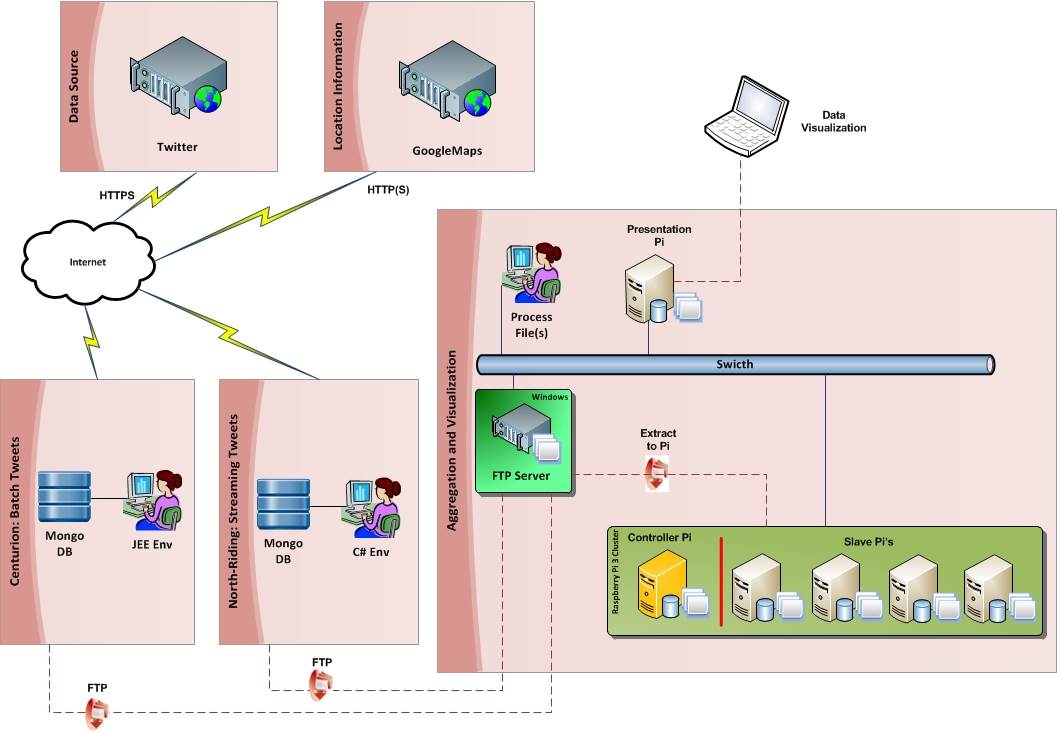
\includegraphics[width=1.15\linewidth]{OM1}}
			\caption{Operational Model: Phyical}
			\label{fig:speciation}
		\end{figure}
	
	
	\subsection{Possible Extensions}
	
	The project used only Twitter as the Big Data source. According to Statista[6], in April 2016 Facebook ranked number one with 1 590 millions of active users, while Twitter recorded 320 millions of active users. Other social media networking sites that were ranked included Integram, WhatApp, WeChat and LinkedIn among others. Most the social networking service provides an API retrieve social media messages or posts. The project chose Twitter as the data source because Twitter's API seemed to be easier to work with. Due to lack of time only one data source was choosen. One of the possible extension in the project lies on the data collection component. The 2 sub-components can be enhanced to support other social media platforms as the data providers.
	\\
	\\
	Other potential extensions to the solution include developing a smart-phone/ tablet App to make the same sort of analytics reports available to a category of user that is always on the move.
	\\
	\\
	The system itself can in future be hooked into LDAP in order to better control user access and security from a central point as well as ease of provision for new users.
	
	%\subsection{Explanation Summary} %--optional
	
	% Risk - large project given to a small company that is running a core part of the company's systems.
	
	%------------------------------------------------
	
	%\subsubsection{Executive Summary}%--optional
	
	
	%\begin{figure}[H] % Example image
	%	\center{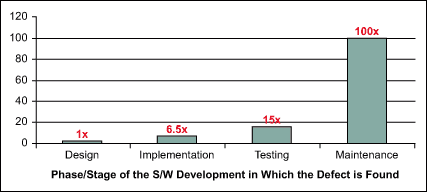
\includegraphics[width=0.55\linewidth]{IBM}}
	%	\caption{Relative Costs to Fix Software Defects (Source: IBM Systems Sciences Institute)}
	%	\label{fig:speciation}
	%\end{figure}
	
	%----------------------------------------------------------------------------------------
	%	CONCLUSION
	%----------------------------------------------------------------------------------------
	
	\section{Conclusion} % Major section
	
	All this hardware and software is available to anybody interested in Big Data processing.\\
	
	The hardware is cheap and the software is free.\
	
	The learning curve in the beginning can be quite steep but is ultimately very rewarding in terms of what can be achieved with so little financial investment.
	
	
	
	
	\newpage
	
	%----------------------------------------------------------------------------------------
	%	BIBLIOGRAPHY
	%----------------------------------------------------------------------------------------
	
	\begin{thebibliography}{99} % Bibliography - this is intentionally simple in this template
		
		\bibitem 1. S. Madam. From Databases to Big Data. IEEE Computer Society, 2012.
	
		%\newblock 
		
		\bibitem 2. V. Kumar, R. Yuvaraj, C. Anusha. Effective Distribution of Large Scale Datasets Clustering Based on MapReduce. 2016.

		
	\end{thebibliography}
	
	\section{Appendices}
	
	%----------------------------------------------------------------------------------------
	
\end{document}